\documentclass[10pt]{article}

\usepackage[margin=1in]{geometry}
\usepackage{amsmath,amssymb,amsthm}
\usepackage{graphicx}
\usepackage{booktabs}
\usepackage{microtype}
\usepackage[numbers,sort&compress]{natbib}
\usepackage{xcolor}
\usepackage[colorlinks=true,linkcolor=blue!60!black,citecolor=blue!60!black,urlcolor=blue!60!black]{hyperref}
\usepackage{caption}
\captionsetup{font=small,labelfont=bf}

\newcommand{\TODO}[1]{\textcolor{red}{[TODO: #1]}}
\newcommand{\loss}{\mathcal{L}}
\newcommand{\R}{\mathbb{R}}

\title{A One-Sided Level-Crossing Budget for Physics-Informed Neural
Networks:\\ Validated Mechanism, Absent Pathology}

\author{%
Gunner Levi Howe\\
Independent Researcher\\
\texttt{gunnerlevihowe@gmail.com}%
}

\date{July 2026}

\begin{document}
\maketitle

\begin{abstract}
Physics-informed neural networks (PINNs) on stiff and unstable PDEs are widely
reported to fail through runaway high-frequency oscillation---most pointedly on the
complex Ginzburg--Landau equation (CGLE), where a recent architecture-level fix
(ASPEN) is premised on a conventional MLP PINN ``catastrophically diverging into
non-physical oscillations.'' We design the natural \emph{loss-level} counterpart: a
one-sided \emph{level-crossing budget}, built on the Kac--Rice/co-area machinery of
our companion work, that penalizes the network field's spatial crossing density only
where it exceeds the physical budget of the solution class. The loss is mesh-free,
FFT-free, evaluated at the collocation points a PINN already uses, costs one spatial
derivative the residual already computes, and is provably inactive---zero loss,
zero gradient---on fields within budget. We validate the mechanism in vitro: on
sparse-data interpolation where a periodic-activation network demonstrably
over-oscillates, the budget clamps the crossing profile to specification and improves
test error on every seed. We then report, with full receipts, a negative result in
vivo: across a faithful reimplementation of the ASPEN benchmark (two input
conventions, up to the full published training depth) and a Benjamin--Feir-unstable
chaotic testbed, the vanilla PINN always fails---but always by \emph{under}-resolving
or decorrelating, never by excess oscillation. Its crossing density sits below the
physical budget at every level, so a one-sided budget is verifiably inert, and
uniform gradient damping is inert or harmful for the same reason. We conclude that
loss-level oscillation suppressors---ours included---address a failure mode whose
prevalence is implementation-sensitive, and we release a crossing-profile diagnostic
that distinguishes over- from under-oscillatory PINN failure in one plot, together
with all code, reference solvers, and raw runs.
\end{abstract}

\section{Introduction}
\label{sec:intro}

Physics-informed neural networks \citep{raissi2019pinn} minimize a PDE residual at
collocation points instead of fitting data on a grid. Their failure modes are by now
a literature of their own \citep{krishnapriyan2021failure,wang2024causal}: stiff
dynamics, chaotic regimes, and long horizons produce solutions that are smooth,
plausible, and wrong---or, in the telling of several recent papers, fields that
\emph{blow up in high frequency}. On the complex Ginzburg--Landau equation (CGLE),
the canonical stiff nonlinear testbed \citep{aranson2002cgle}, the ASPEN
architecture \citep{aspen2025} is motivated by exactly this claim: a conventional
MLP PINN ``develops spurious, high-frequency oscillations that grow in time,
rendering the prediction physically meaningless.''

If the pathology is excess oscillation, there is a natural \emph{loss-level},
architecture-agnostic counterpart to spectral architecture fixes. In companion work
on implicit neural representations \citep{howe2026levelcrossing} we turned the Rice
level-crossing density \citep{rice1944,kac1943}---the number of times a field
crosses a level per unit length, a closed-form spatial proxy for frequency content
\citep{kedem1986zerocrossings}---into a differentiable training signal via the
co-area formula and a smoothed Monte-Carlo estimator. There, the loss \emph{demands}
crossings that spectrally biased networks under-produce. Here we flip its sign: a
\textbf{one-sided crossing budget} that penalizes the field only where its crossing
density \emph{exceeds} what the physics allows. One mechanism, both directions.

The budget has three properties tailored to PINNs. It is evaluated pointwise at the
scattered collocation points themselves---no grid, no FFT, exactly where
frequency-domain penalties are awkward. It reuses the spatial derivative the residual
loss already computes, so its marginal cost is one kernel evaluation. And it is
\emph{one-sided by construction}: on a field within budget it contributes zero loss
and, provably, zero gradient---it cannot push a smooth field toward oscillation, the
failure it is designed to prevent. Budgets come from three sources of decreasing
strength: a reference spectral simulation, a closed-form physics prior (for a
monotone-front class, each level is crossed once per front), or a single scalar cap.

\paragraph{Pre-registered honesty.} This study was gated and kill-conditioned in
advance: the mechanism had to demonstrably steer crossing profiles (established in
the companion work and re-verified in vitro here), the vanilla failure had to
reproduce, and---the condition that fired---the failure had to actually \emph{be}
the excess-oscillation pathology. We report what happened, in full.

\paragraph{Contributions.}
(1)~\emph{The loss}: a validated, one-sided, physically calibrated crossing-density
budget with three budget sources and a zero-gradient-under-budget guarantee
(Section~\ref{sec:method}).
(2)~\emph{An in-vitro positive control}: on sparse-data interpolation with a
periodic-activation network---a setting that genuinely over-oscillates---the budget
clamps the crossing profile to specification and improves test error on every seed
(Section~\ref{sec:invitro}).
(3)~\emph{A receipted negative result}: on a faithful reimplementation of the ASPEN
CGLE benchmark (both raw and normalized inputs, 30k and the full published 100k
iterations) and on a Benjamin--Feir-unstable chaotic CGLE testbed, vanilla PINNs
fail \emph{under}-oscillatorily in every run; the budget---and uniform gradient
damping---are verifiably inert on such failures (Section~\ref{sec:invivo}).
(4)~\emph{A diagnostic}: the measured crossing profile against the physical budget
separates over- from under-oscillatory failure in a single plot, and would have
identified the mismatch between pathology and remedy before any stabilizer was
trained (Section~\ref{sec:diagnostic}).

\section{Related work}
\label{sec:related}

\paragraph{PINN failure modes and schedules.} \citet{krishnapriyan2021failure}
characterize why residual training fails on seemingly simple PDEs and propose
curriculum/seq2seq regimes; \citet{wang2024causal} enforce temporal causality
through residual weighting. Both address the \emph{propagation} failure---early
times fit, later times lost---which is precisely the mode we observe on the CGLE
front benchmark. Architecture-level spectral remedies include Fourier features
\citep{tancik2020fourier}, ASPEN's adaptive spectral layer \citep{aspen2025}, and
multi-scale SIREN variants for Ginzburg--Landau dynamics
\citep{chrisnanto2026sirenpinn}.

\paragraph{Crossing statistics.} The Rice formula and its co-area generalization
\citep{rice1944,kac1943,adler2007random,azais2009level} give the expected level-set
measure of a field; zero-crossing rates as frequency surrogates are classical
\citep{kedem1986zerocrossings}. Our companion paper \citep{howe2026levelcrossing}
develops the differentiable estimator and studies the \emph{demand} direction for
implicit neural representations; to our knowledge no prior work uses a crossing
\emph{budget} as an anti-oscillation regularizer for PINNs---and this paper's
finding is that on the tested CGLE regimes, nothing does, because the pathology it
targets did not occur.

\section{The one-sided crossing budget}
\label{sec:method}

Let $f_\theta$ be one real component of the PINN field (we budget $\mathrm{Re}\,A$
and $\mathrm{Im}\,A$ separately). With the smoothed Monte-Carlo crossing density of
the companion work,
\begin{equation}
\hat c_\varepsilon(u) \;=\; \frac{1}{N}\sum_{i=1}^{N}
\delta_\varepsilon\!\bigl(f_\theta(x_i,t_i)-u\bigr)\,
\bigl|\partial_x f_\theta(x_i,t_i)\bigr|,
\label{eq:estimator}
\end{equation}
evaluated at the PDE collocation points $(x_i,t_i)$ (Latin hypercube over
space-time; $\partial_x f_\theta$ is shared with the residual computation), the
budget loss at fixed levels $u_1,\dots,u_L$ spanning the solution class's amplitude
range is
\begin{equation}
\loss_{\mathrm{budget}}
= \frac1L \sum_{j=1}^{L}
\left[\frac{\mathrm{relu}\bigl(\hat c_\varepsilon(u_j) - b_j\bigr)}
{b_j + \bar b}\right]^2 ,
\qquad \bar b = \tfrac1L\textstyle\sum_j b_j .
\label{eq:budget}
\end{equation}
Levels are \emph{fixed a priori}---a PINN has no ground-truth field from which to
take quantiles---and the one-sidedness is mandatory: early in training the field is
smooth, and a symmetric matching loss would \emph{pump oscillation in}, the exact
failure being prevented. Under budget, \eqref{eq:budget} is identically zero on an
open set of fields, so its gradient vanishes as well; our released unit tests verify
both properties, along with the estimator's agreement with exact crossing counts and
the Rice formula (within $5\%$ and $10\%$ respectively, reproduced from the
companion work).

\paragraph{Budget sources.} (a)~\emph{Reference simulation}: per-level crossing
densities measured on a spectral/finite-difference reference of the same solution
class (95th percentile over time, $\times1.5$ slack)---the strongest budget, but it
presumes a solver, which we state plainly. (b)~\emph{Physics prior}: for the
monotone-front class of the ASPEN benchmark, a front crosses each level in its range
once per passage, so $b_j = m/L_{\mathrm{dom}}$ with a small allowance $m$ for shed
transients---no simulation, no spectrum. For statistically stationary classes the
Rice form $b \approx \tfrac1\pi\sqrt{\lambda_2/\lambda_0}$ from the physical
spectrum plays the same role. (c)~\emph{Scalar cap}: one number for all levels.

\paragraph{The profile as a diagnostic.}
\label{sec:diagnostic}
Independently of training, comparing the \emph{measured} profile
$\hat c_\varepsilon(u)$ of any trained field against $b_j$ classifies the failure
mode: profile above budget $\Rightarrow$ excess oscillation (the budget's patient);
profile below budget with large error $\Rightarrow$ under-resolution or
decorrelation, for which oscillation suppressors of any kind are the wrong medicine.
Every conclusion in Section~\ref{sec:invivo} is legible in this one plot
(Figure~\ref{fig:taxonomy}).

\section{In vitro: the mechanism works where its pathology exists}
\label{sec:invitro}

Before the PDE setting, we verify the budget on a problem that demonstrably
over-oscillates: a SIREN \citep{sitzmann2020siren} ($\omega_0{=}30$, width 128,
3 hidden layers) fit to 40 random samples of a smooth signal
$y = \tanh(3x) + 0.3\sin(2\pi x)$ on $[-1,1]$. The physics-prior budget allows
$m{=}6$ crossings per level over the domain ($b{=}3$ per unit length). Across three
seeds, the MSE-only network exceeds the budget (peak crossing density $3.4$--$4.3$)
and interpolates with spurious oscillation; adding \eqref{eq:budget} at weight $1$
clamps the peak profile to $2.6$--$2.7$---strictly within budget---and
\emph{improves} dense-grid test MSE in every seed ($0.0233\!\to\!0.0198$,
$0.0274\!\to\!0.0231$, $0.1099\!\to\!0.0649$). The mechanism does exactly what it
claims when excess crossings exist (Figure~\ref{fig:invitro}).

\section{In vivo: the pathology does not show up}
\label{sec:invivo}

\subsection{Testbeds and protocol}

\paragraph{ASPEN front benchmark (faithful reimplementation).} CGLE
$\partial_t A = A + (1+ib)\partial_{xx}A - (1+ic)|A|^2A$ with $b{=}0.5$,
$c{=}-1.3$, $x\in[-10,7.5]$, $t\in[0,10]$, $A(x,0)=\tanh(-x)$, Dirichlet ends
\citep{aspen2025}: a stiff domain-wall relaxation. Vanilla PINN: $8{\times}40$ tanh
MLP, Adam $10^{-3}\!\to\!10^{-4}$, $20{,}000$ residual + $1{,}000$ IC + $1{,}000$
BC Latin-hypercube points, $w_{\mathrm{res}}{=}1$, $w_{\mathrm{ic,bc}}{=}100$---%
ASPEN's published configuration. Reference: method-of-lines RK4 at their
$\Delta t{=}10^{-4}$, $N_x{=}1024$, grid-convergence verified. We run both
normalized-input and raw-coordinate variants, at 30k iterations (3 seeds) and at
the full published 100k depth (both variants, seed 0).

\paragraph{Benjamin--Feir-unstable testbed.} The front benchmark is BF-stable
($1+bc = 0.35 > 0$); genuine broadband dynamics needs the unstable regime. We add
periodic CGLE with $b{=}2$, $c{=}-1.2$ ($1+bc = -1.4$: phase turbulence), $L{=}64$,
ETDRK4 reference \citep{kassam2005etdrk4} run to the attractor, PINN horizon
$T{=}5$ from an attractor state, periodicity hard-wired through Fourier coordinate
embedding so no BC loss is needed.

\paragraph{Metrics.} Relative $L_2$ against the reference on its space-time grid;
radially banded spatial-spectrum error; the crossing profile of
Section~\ref{sec:diagnostic}; temporal turning-point rates.

\subsection{Vanilla failure, wrong disease}

On the front benchmark the vanilla PINN fails reproducibly---relative $L_2$
$0.867\pm0.016$ over three seeds at 30k iterations, physically useless---but the
failure is \emph{propagation loss}, not oscillation: error grows from $0.10$
($t{<}2$) to $0.76$ ($t{>}5$), amplitudes stay bounded ($\max|A| = 1.05$),
temporal turning-point rates sit \emph{below} the reference's, high spatial bands
carry near-zero excess energy, and the crossing profile lies \emph{under} the
physical budget at every level (Figure~\ref{fig:taxonomy}, left). Raw-coordinate
inputs reproduce the same signature ($0.879$). At the full published 100k depth
the story sharpens rather than changes: the normalized variant improves
monotonically to $0.555$ and the raw variant to $0.581$---slow convergence toward
a still-poor solution, with the crossing profile peaking at $0.19$ against a
budget of $0.43$ and high-band spectral excess of $10^{-3}$. There is no depth at
which oscillation appears. On the BF-unstable testbed the vanilla PINN
\emph{diverges} in relative $L_2$ ($0.63\!\to\!1.31$ over training)---but by
progressive decorrelation toward an over-smoothed field: its crossing density
($0.046$ per unit at mid levels) is a third of the reference's ($0.132$), i.e.\ the
network has \emph{fewer} waves than the physics, while its amplitude stays in
$[0.75, 1.2]$. In no run, on no testbed, at no depth, did any field exceed its
crossing budget.

\begin{table}[t]
\centering
\caption{\textbf{In-vivo results.} Relative $L_2$ against the reference (mean
$\pm$ s.d.; seed counts in brackets). Every configuration fails identically:
the budget never has anything to clamp, and damping has nothing to damp.}
\label{tab:p2main}
\begin{tabular}{lcc}
\toprule
 & front benchmark & BF-unstable testbed \\
Config & rel.\ $L_2$ [seeds] & rel.\ $L_2$ [seeds] \\
\midrule
vanilla PINN & 0.867 $\pm$ 0.016 [3] & 1.311 [1] \\
+ budget (reference sim) & 0.866 $\pm$ 0.015 [3] & 1.306 [1] \\
+ budget (physics prior) & 0.875 $\pm$ 0.021 [3] & -- \\
+ budget (scalar cap) & 0.866 $\pm$ 0.015 [3] & -- \\
+ gradient damping (best $w$) & 0.858 [1] & 1.323 [1] \\
\bottomrule
\end{tabular}
\end{table}

\subsection{Consequences: budget and dampers are inert}

Because every failure is under-oscillatory, the one-sided budget is inactive by
construction---and the receipts are as literal as receipts get. On the front
benchmark, budget-augmented training lands within noise of vanilla for all three
budget sources (Table~\ref{tab:p2main}); on seed~1 the budget-ref trajectory is
\emph{bit-identical} to vanilla ($0.8617398766$ in both cases): the one-sided term
never activated, its gradient was exactly zero, and the two optimizations
coincide to machine precision. On other seeds the shed initial transient briefly
exceeds the central-level budgets, the term activates transiently, and endpoints
shift by at most $0.016$ relative $L_2$ (largest for the tightest budget, the
physics prior)---activation without consequence, since the eventual failure is
not oscillatory. On the chaotic testbed the triple
is $1.311$ (vanilla), $1.306$ ($+$budget), $1.323$ ($+$gradient damping): all
identical within noise. Uniform gradient damping, the natural null control, is
likewise inert on the front benchmark ($0.858$ at its best weight, seed~0,
vs.\ vanilla $0.850$) and mildly harmful on the chaotic one---there is no excess
gradient energy to damp, only missing structure. The sober, useful reading:
\emph{loss-level oscillation suppressors of any flavor cannot help a PINN whose
failure is under-resolution}; the remedies that address propagation failure
(causal weighting, curricula, architecture) live on a different axis.

\subsection{On the discrepancy with the published failure mode}

Our reimplementation follows ASPEN's published configuration in equation,
parameters, domain, conditions, architecture, sampling, loss weights, optimizer,
schedule, and depth; we additionally varied input normalization and doubled the
testbed with a BF-unstable regime. We could not elicit growing high-frequency
oscillation in any of these runs. We do not conclude that the published observation
is wrong---initialization schemes, precision, framework defaults, or unreported
details can all select among PINN failure branches. We conclude that the
\emph{prevalence} of the oscillatory branch is implementation-sensitive, which
matters for how the community motivates oscillation-suppressing machinery: a
stabilizer aimed at a branch that a given stack never visits will measure as inert,
and the crossing-profile diagnostic of Section~\ref{sec:diagnostic} detects this
mismatch \emph{before} any stabilizer is trained.

\section{Discussion and limitations}
\label{sec:discussion}

\paragraph{What survives.} The budget mechanism itself is validated: one-sided,
provably silent under budget, and effective in vitro where excess crossings exist.
The crossing-profile diagnostic is, to our knowledge, new to PINN failure analysis
and costs one forward/backward pass. The negative result is bounded and specific:
1D CGLE, front and phase-turbulent regimes, the published protocol family, our
stack.

\paragraph{What we did not test.} Deep defect chaos ($|A|\!\to\!0$ defects), other
stiff families (Kuramoto--Sivashinsky, reaction--diffusion with sharp fronts),
2D/3D, and PINN variants whose training dynamics differ enough to visit the
oscillatory branch (e.g., very high-frequency Fourier features with aggressive
learning rates---the regime where our in-vitro patient lives). If a stack does
exhibit budget-violating fields, Section~\ref{sec:invitro} is direct evidence the
clamp then works; finding a PDE setting where that occurs organically is the open
question this paper hands to the community, receipts included.

\section{Conclusion}

We built the loss that the ``catastrophic high-frequency divergence'' narrative
calls for, proved it behaves as specified in both activation and silence, and then
could not find the disease it cures in the very setting that motivates it. Both
halves are the contribution: a validated one-sided crossing budget---the cap
direction of a mechanism whose demand direction helps implicit neural
representations---and a documented, reproducible absence, with a one-plot diagnostic
that tells any practitioner which failure branch their PINN is actually on before
they reach for a stabilizer.

\paragraph{Reproducibility.} Code, both reference solvers, all raw run JSONs, and
the unit tests are public at \url{https://github.com/gunnerhowe/Research}
(directory \texttt{kac-rice}; Phase-2 modules \texttt{cgle.py}, \texttt{pinn.py},
\texttt{crossing.py::CrossingBudgetLoss}, runner
\texttt{experiments/run\_phase2.py}). Single consumer workstation (RTX~3080).

\bibliographystyle{plainnat}
\bibliography{references}

\appendix

\section{Reproducibility}
\label{app:repro}

Code, both reference solvers, all raw run JSONs, and unit tests:
\url{https://github.com/gunnerhowe/Research} (directory \texttt{kac-rice}).
Environment: Python 3.13.6, PyTorch 2.7.1, NumPy 2.4.4, SciPy 1.17.0; one
consumer workstation (16-core CPU / RTX~3080, shared with unrelated jobs, so
wall-clock is never a reported metric here).

\paragraph{Commands.} Correctness tests (residual vanishes on exact CGLE
plane waves; solver grid convergence; budget one-sidedness including the
zero-gradient property): \texttt{python tests/test\_phase2.py}. The reference
solutions are computed once and cached
(\texttt{results/phase2/reference*.npz}). Experiment suites map to the paper
as follows, all via \texttt{experiments/run\_phase2.py} (resume-safe):
\texttt{--suites exp3 exp4} (Table~1 front rows; Figs.~1, 3),
\texttt{--suites exp5} (damping row), \texttt{--suites chaos}
(BF-unstable column), \texttt{--suites diag diag100k} (input-convention and
100k-depth receipts), \texttt{--suites invitro} (Section~4, Fig.~2). Figures
and the table regenerate with
\texttt{python experiments/make\_figures\_phase2.py}.

\paragraph{Seeds and receipts.} Seeds $0$--$2$ (front benchmark and in
vitro); the chaotic testbed and 100k-depth runs use seed $0$ and are labeled
with their seed counts in Table~1. Every claim in Section~5 cites a specific
recorded run; the bit-identity claim can be checked directly against
\texttt{exp3\_g1.json} and \texttt{exp4\_g1.json} (seed~1, full precision).

\section{Hyperparameters}
\begin{table}[h]
\centering
\caption{Phase-2 hyperparameters.}
\begin{tabular}{ll}
\toprule
Budget loss & $L{=}16$ levels on $[-1.05,1.05]$; $\varepsilon{=}0.08$; weight $1.0$ \\
Budget sources & ref.\ sim (q95 $\times$1.5 slack); physics prior $m{=}4$; scalar cap \\
Vanilla PINN & $8\times40$ tanh; Adam $10^{-3}\to10^{-4}$ at half-depth \\
Collocation & $20{,}000$ res.\ + $1{,}000$ IC + $1{,}000$ BC, Latin hypercube \\
Chaotic testbed & $b{=}2$, $c{=}-1.2$, $L{=}64$, $T{=}5$, periodic embedding, 4 harmonics \\
In vitro & SIREN $\omega_0{=}30$, 40 samples, budget $m{=}6$ over $[-1,1]$ \\
Seeds & 3 per configuration \\
\bottomrule
\end{tabular}
\end{table}

\begin{figure}[h]
\centering
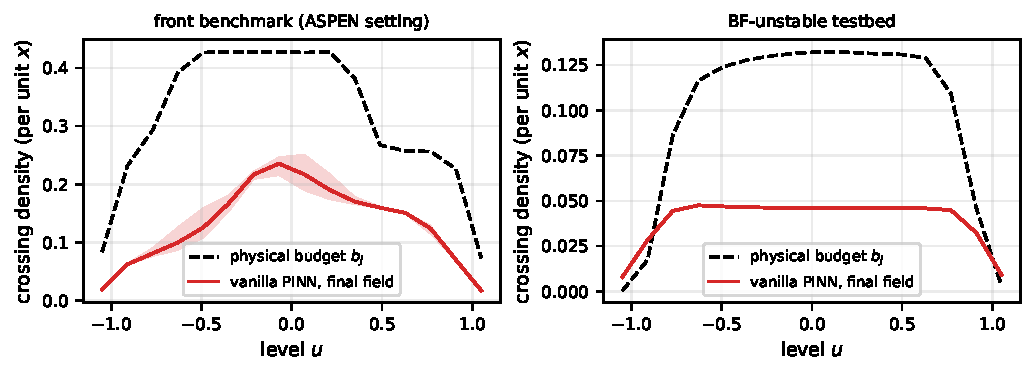
\includegraphics[width=\linewidth]{figs/p2_taxonomy.pdf}
\caption{\textbf{The diagnostic in action}: measured crossing profiles versus
physical budgets for the front benchmark (left; band = min--max over 3 seeds)
and the BF-unstable testbed (right). Every failed vanilla field sits
\emph{below} budget---the under-oscillatory branch, on which one-sided budgets
are by design inert.}
\label{fig:taxonomy}
\end{figure}

\begin{figure}[h]
\centering
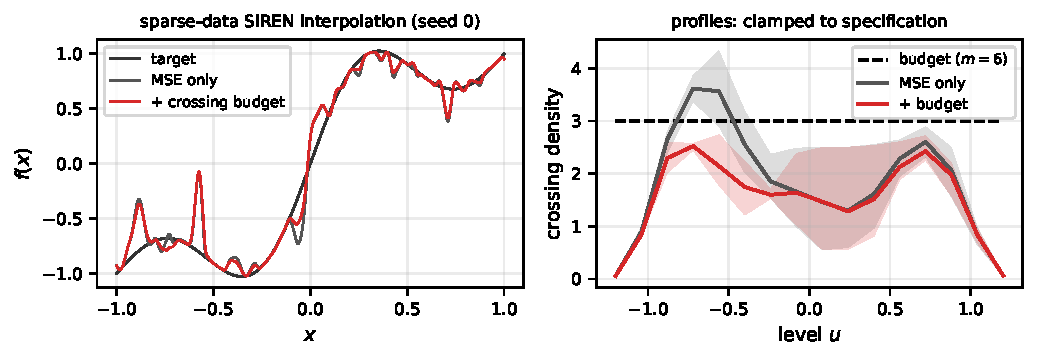
\includegraphics[width=.7\linewidth]{figs/p2_invitro.pdf}
\caption{\textbf{In-vitro positive control}: sparse-data SIREN interpolation
(left: seed-0 reconstructions; right: crossing profiles, min--max band over 3
seeds). MSE-only over-oscillates beyond budget; the one-sided budget clamps the
profile within specification and improves test error on all seeds.}
\label{fig:invitro}
\end{figure}

\end{document}
